\chapter{The Compact Muon Solenoid}
\label{chap:detector}

\section{Introduction}

The Large Hadron Collider (LHC) at CERN is a 27\,km hadron accelerator and collider with a design centre-of-mass energy of 14\,TeV~\cite{LHC}.
Its purpose is to provide collisions sufficient in energy and number to precisely probe physics at the electroweak scale.
Four detectors, one of which is the Compact Muon Solenoid (CMS), are situated around the LHC ring.
CMS is a general-purpose detector designed to precisely measure a wide range of physics objects.
Together, the LHC and CMS facilitate a wide-ranging program of physics studies, from SM precision measurements to dark matter searches, 
and including exploration of electroweak symmetry breaking via production of the Higgs boson.
This chapter will describe the design and operation of both the LHC and the CMS detector.

\section{The Large Hadron Collider}

The LHC is situated in the tunnel that previously housed the Large Electron Positron collider (LEP)~\cite{LEP}, 
around 100\,m below ground across the French-Swiss border near CERN.
It is the final machine in a series of accelerators which form the CERN accelerator complex~\cite{CERNcomplex}; 
these  act as the injection system for the LHC.
The two counter-circulating beams cross at four interaction points, at each of which a detector is situated.
Directly opposite CMS is a second general purpose detector, ATLAS~\cite{ATLAS}, 
whose physics objectives are identical to those of CMS but whose design and operation are independent. 
The other two detectors, LHCb~\cite{LHCb} and ALICE~\cite{ALICE}, focus on flavour and heavy-ion physics respectively.
Whilst the LHC is capable of producing heavy ion collisions in addition to proton-proton collisions, 
the remainder of this section will be dedicated to its proton-proton operations.
A schematic of the full CERN accelerator complex and the LHC experiments is shown in Figure~\ref{fig:detector_CERNschematic}.
The operation of the LHC and the data it has accumulated so far is described in detail below.

%FIXME this is too small
\begin{figure}[h!]
  \centering
  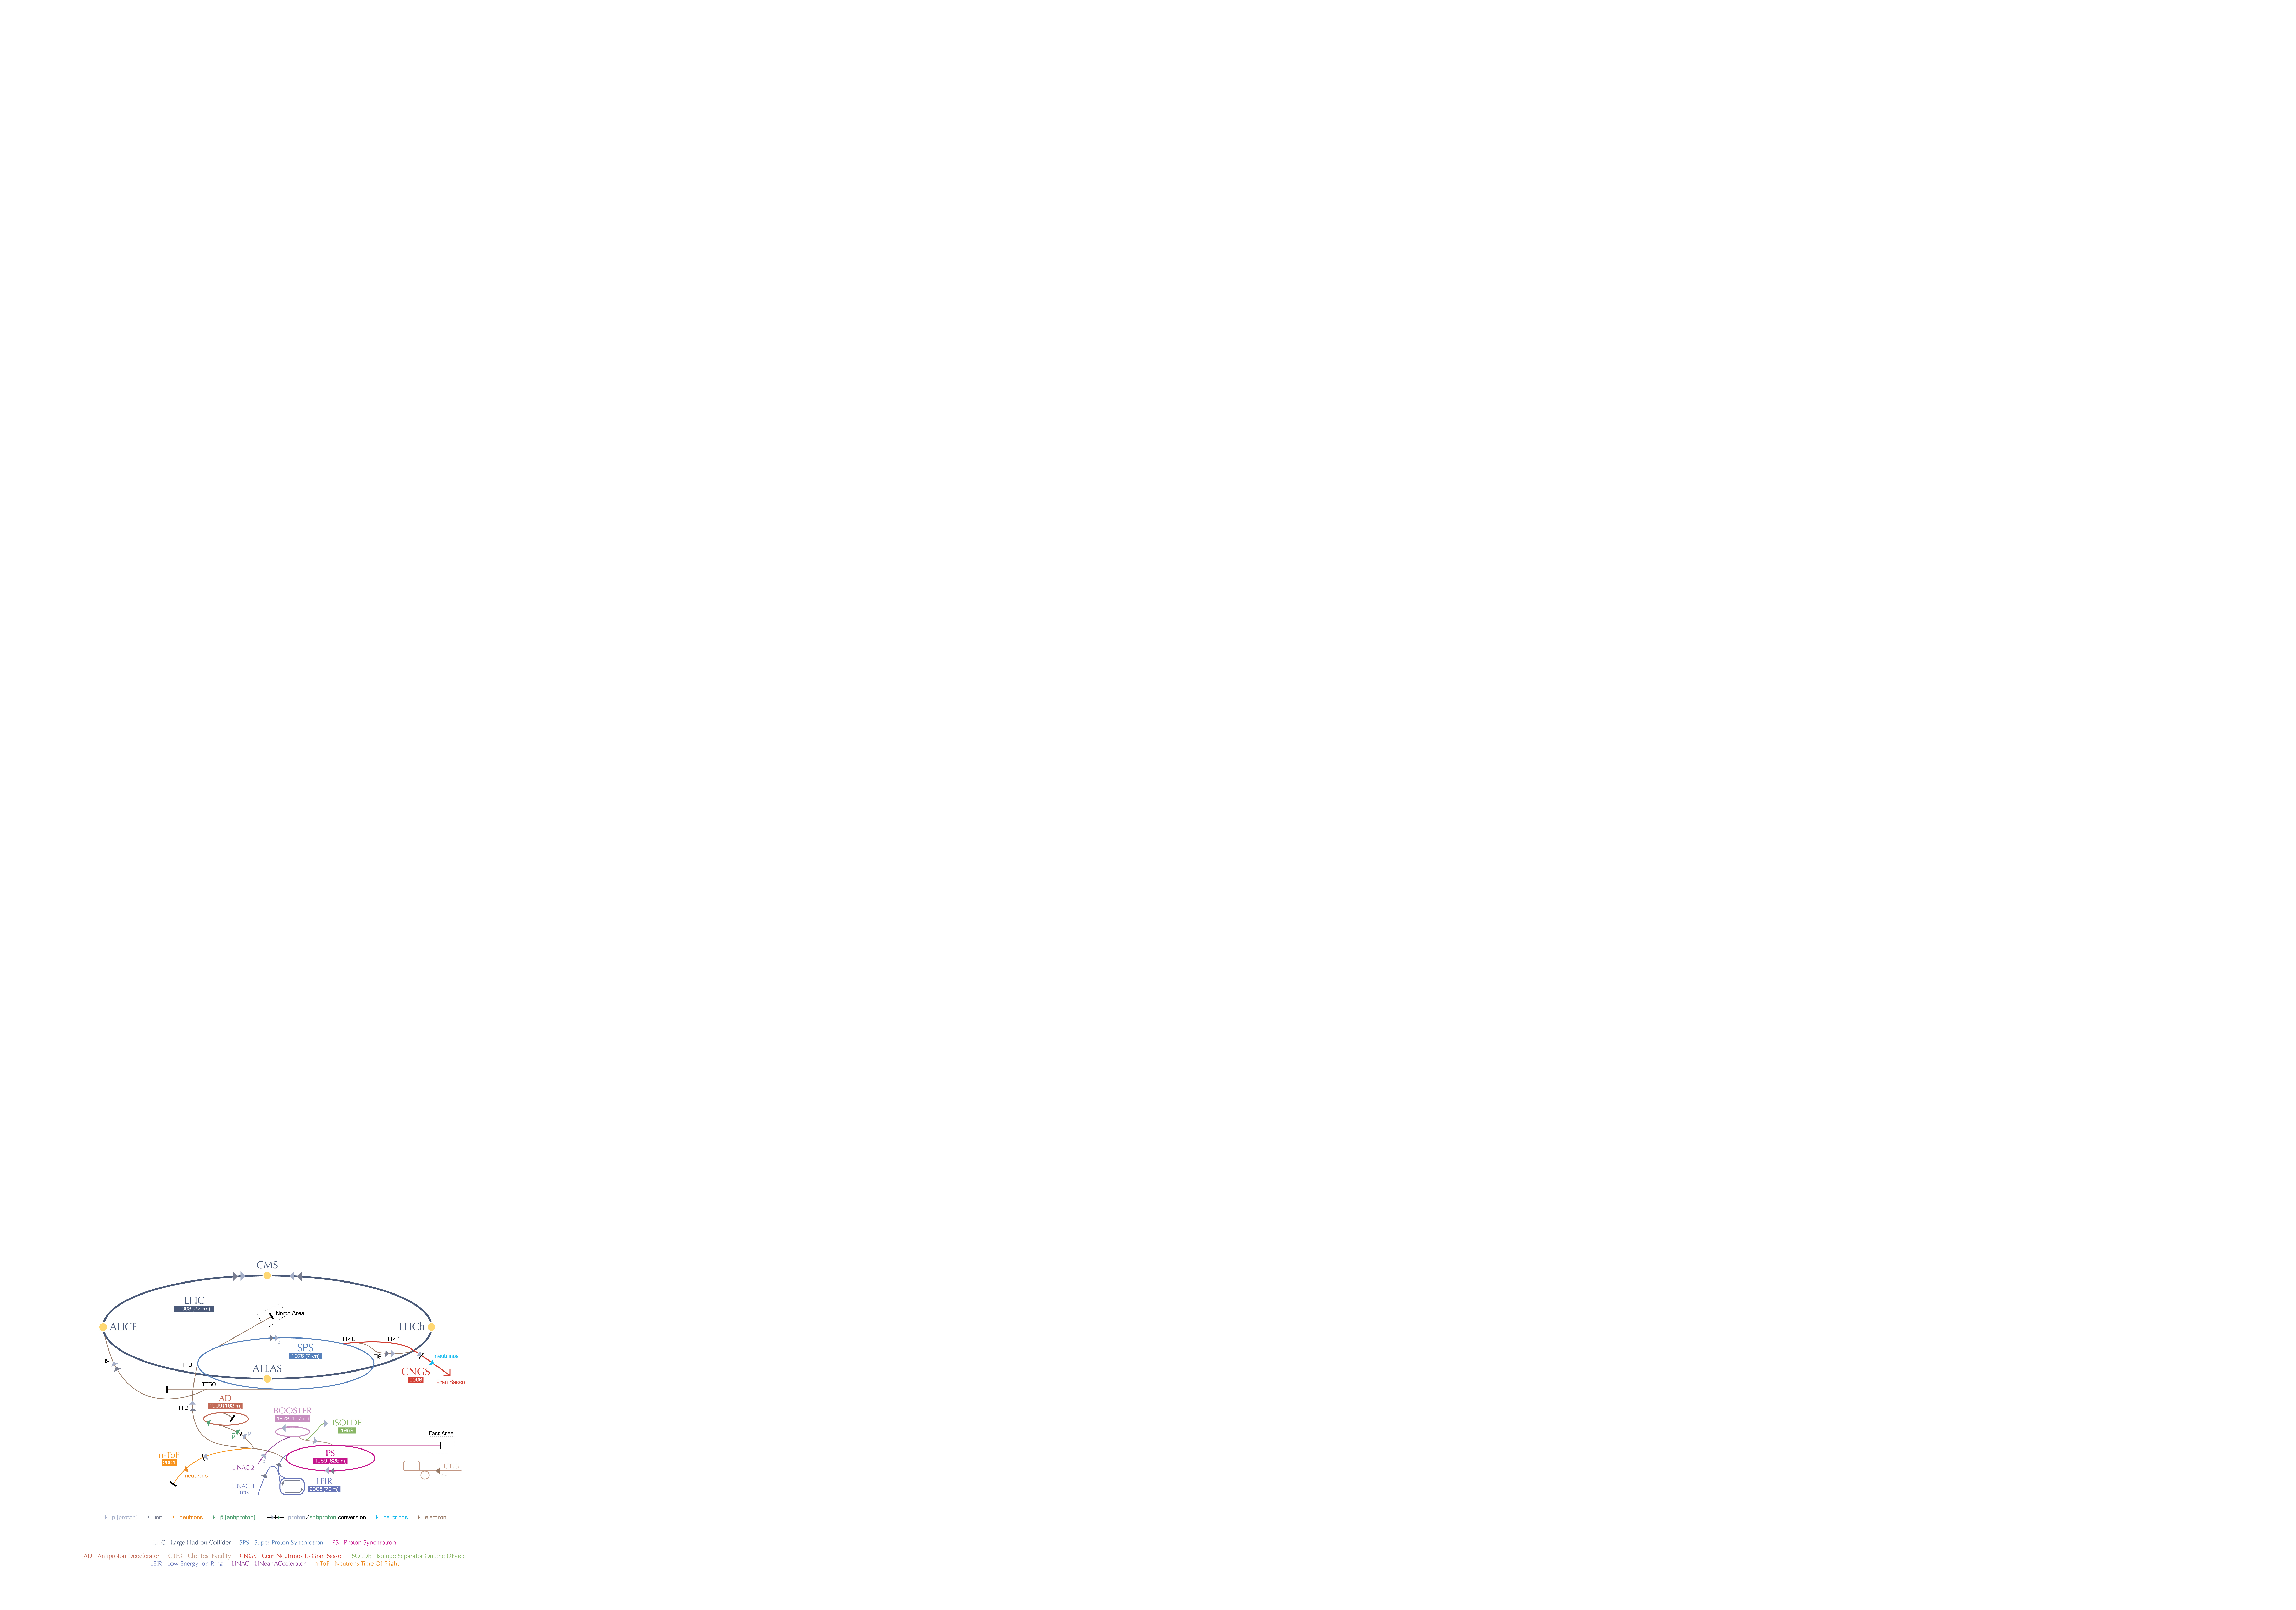
\includegraphics[width=\textwidth]{Figures/Detector/CERNschematic.pdf}
  \caption[The CERN accelerator complex.]
  {The LHC and its experiments within the CERN accelerator complex.
  Figure taken from Ref.~\cite{CERNcomplex}.}
  \label{fig:detector_CERNschematic}
\end{figure}

The LHC design parameters allow for proton-proton collisions to occur at a maximum centre-of-mass energy of 14\,TeV 
with an instantaneous luminosity of up to $1/,\times\,10^{34}\,\textrm{cm}^{-2}\,\textrm{s}^{-1}$.
Prior to being injected into the LHC beam pipes, bunches of protons pass are accelerated in several stages. 
First, protons are obtained by stripping the electrons from hydrogen atoms using a strong electric field.
The protons produced are then accelerated up to an energy of 50 MeV by Linear Accelerator 2 (LINAC 2).
LINAC 2 leads into the Proton Synchrotron Booster (PSB), where they reach an energy of 1.4 GeV before passing into the Proton Synchrotron (PS).
Here the beam is accelerated up to 25 GeV before being transferred to the Super Proton Synchrotron (SPS).
The SPS is the last step before the protons enter the LHC itself at an energy of 540 GeV.
Therefore the LHC is responsible for the final acceleration from 540 GeV to the full energy.
Thus far, the energy reached for stable operation is 6.5\,TeV per beam; 
the full design energy is expected to be achieved in future, beginning in 2021.

The key components of the LHC are its 1232 main dipole magnets, 392 main quadrupole magnets and 16 radiofrequency (RF) cavities.
Superfluid helium cools the dipole magnets to 1.9K, at which temperature they produce the 8.3T magnetic field required to keep the beams in circular orbit.
Quadrupole magnets are used principally to focus the beams near the interaction points, which increases the probability of a high-energy proton-proton collision.
The RF cavities deliver an accelerating field of 5MV/m at a frequency of 400MHz, and furthermore maintain the shape of the 2808 proton bunches per beam.
Collisions occur at the four interaction points, where bunches are induced to collide at a frequency of 25ns. 

The operation of the LHC to date has comprised two separate runs.
Run~1 commenced in 2010 with $\sqrt{s}$ = 7\,TeV, continuing into 2011 at the same centre-of-mass energy to give a total of 6.1\,\fb of data.
In 2012 this was increased to 8\,TeV, and a total of 23.3\,\fb of data were collected.
Analyses based upon this Run~1 dataset were able to discover the Higgs boson~\cite{ATLASdiscovery,CMSdiscovery}.
After a shutdown for upgrades to the machine, Run~2 ran from 2015 to 2018 at a constant 13\,TeV centre-of-mass energy.
The LHC was able to exceed its design luminosity in each of the years, eventually levelling the luminosity at $2\times10^{34}\,\textrm{cm}^{-2}\,\textrm{s}^{-1}$ for the majority of 2018 operations.
A number of additional inelastic proton-proton collisions in addition to a collision of interest, known as pileup, occur at a rate proportional to the instantaneous luminosity.
The mean number of pileup events was 27 per bunch crossing in 2016, and 37 in both 2017 and 2018 data-taking.
Figure \ref{fig:detector_Run1andRun2lumi} summarises the data collected in each year.
%The latest \Hgg results on which this thesis is based have utilised the 2016 and 2017 datasets; 
%plans for the final Run 2 result combining the 2016-2018 datasets are described in Chapter ~\ref{chap:conclusion}.
%Furthermore, future upgrades to both the LHC and the CMS detector are discussed in Chapter~\ref{chap:hgcal}.
%Gavin says not relevant here

\begin{figure}[h!]
  \centering
  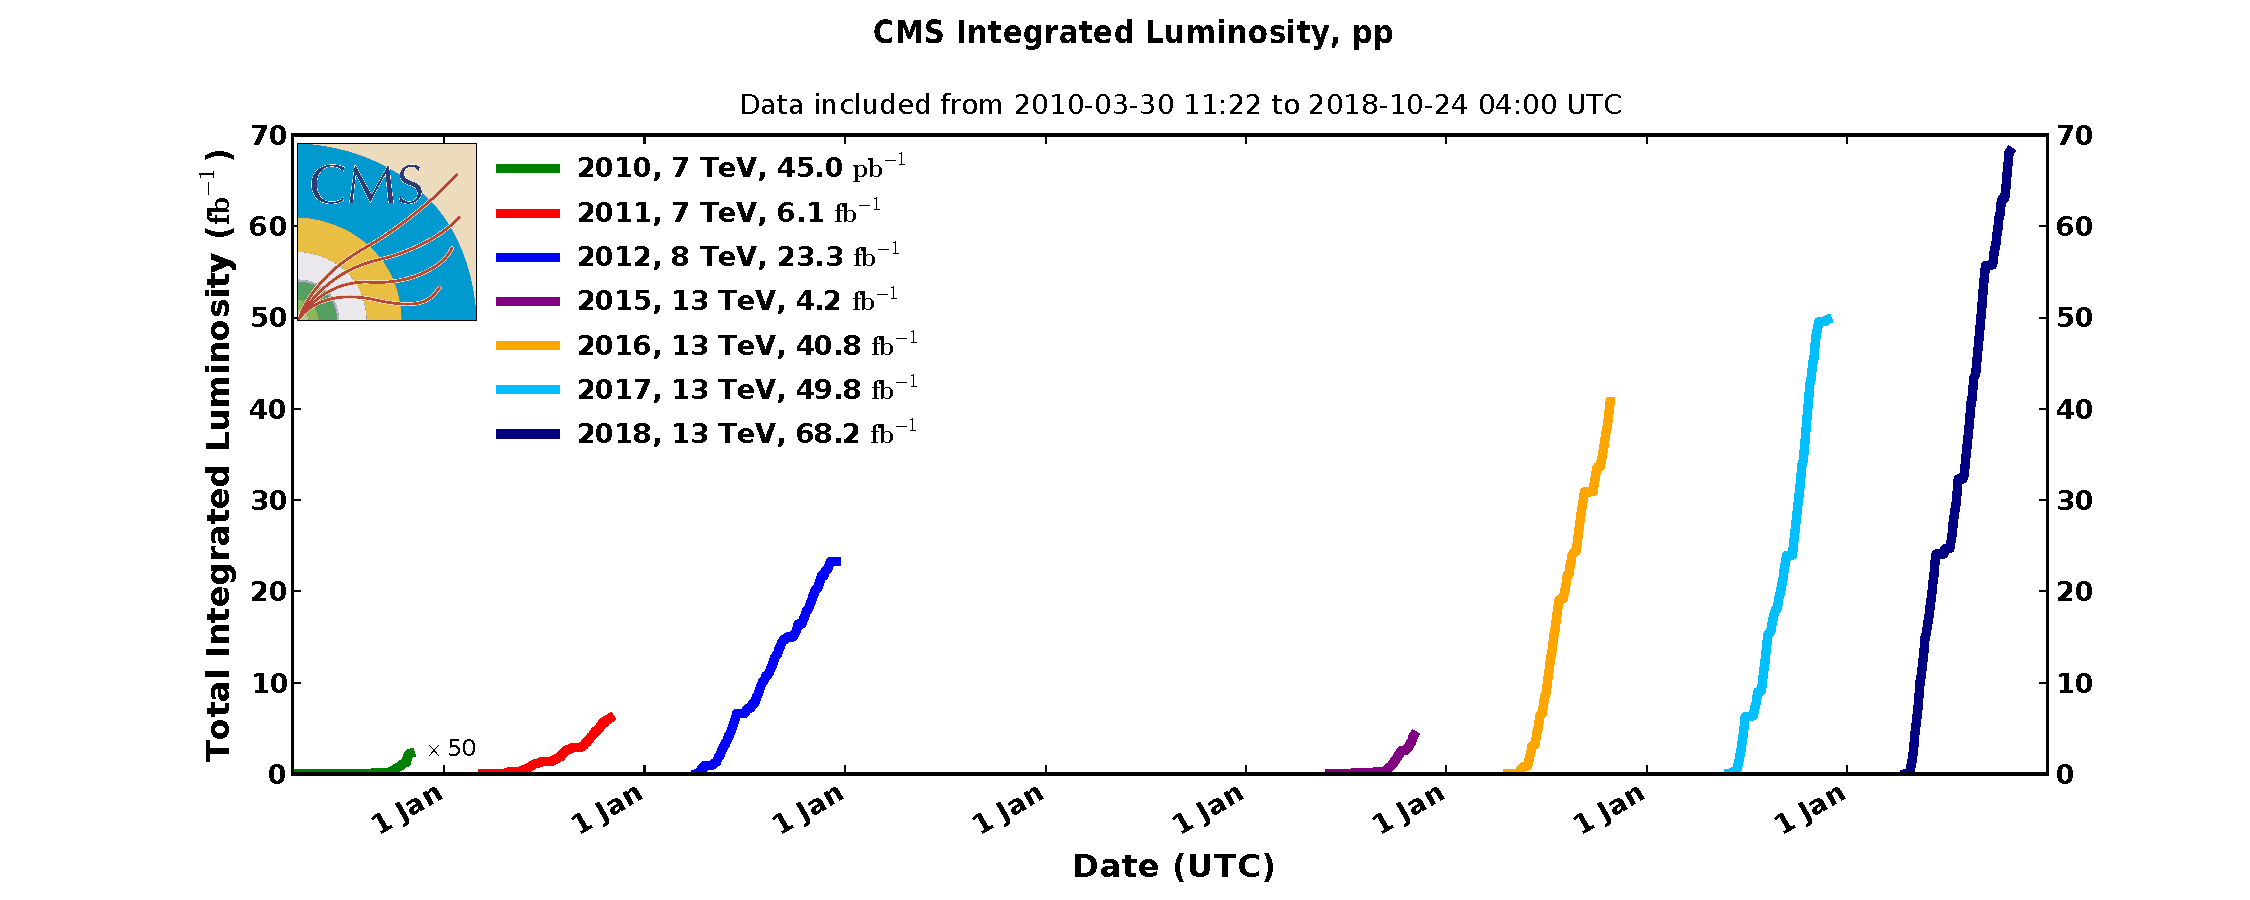
\includegraphics[width=\textwidth]{Figures/Detector/Run1andRun2lumi.pdf}
  \caption[LHC integrated luminosity and centre-of-mass energy per year.]
  {The integrated luminosity and centre-of-mass energy for each year of LHC operation.
  Figure taken from Ref.~\cite{CMSLumiPublic}.}
  \label{fig:detector_Run1andRun2lumi}
\end{figure}

\section{The CMS detector}

CMS is a general purpose detector~\cite{CMSdetector} designed to capture the full range of objects required to achieve the goals of the LHC physics programme.
The apparatus must be able to cope with high pileup at a very high rate; around 1000 charged particles are produced every 25\,ns.
Fine spatial and temporal granularity is required to obtain the sufficiently low occupancy necessary to perform well in these conditions.
The resulting quantity of detector channels presents challenges for the detector electronics.
Furthermore, the detector and its electronics must withstand high doses of radiation and fluence.

In addition to these technical constraints, CMS has four key physics requirements.
These are summarised as:
\begin{itemize}
  \item{\textbf{Muon identification and resolution:}
  muons must be identified and well-measured over a wide range in energy and angle, 
  with good dimuon mass resolution and the capability to accurately determine their charge.
  This is very important for Higgs searches, particularly in the $ZZ$ decay channel.}
  \item{\textbf{Charged particle measurement:}
  good momentum resolution along with efficient reconstruction and triggering on $\tau$ leptons and $b$-jets.
  Excellent jet reconstruction is essential in the majority of physics measurements.}
  \item{\textbf{Electromagnetic energy resolution:}
  good energy resolution and isolation for electrons and photons, whilst maintaining high acceptance.
  These properties are vital for Higgs measurements, especially in the diphoton decay channel.}
  \item{\textbf{Missing energy resolution:}
  accurate missing energy calculation and mass resolution of dijet objects.
  Missing energy is the key signature in many analyses searching for supersymmetry.}
\end{itemize}

The design of CMS fulfils each of these requirements.
The hermetic detector is cylindrical in shape, housing the eponymous 4\,T solenoidal magnet in the central section.
Its other key components include the silicon tracker, homogeneous crystal electromagnetic calorimeter (ECAL) and a sampling hadronic calorimeter (HCAL).
The tracker and calorimeters lie inside the bore of the magnet coil; the muon detection system is instead interleaved with the return yoke.
Each of these subsystems is displayed in Figure~\ref{fig:detector_CMSschematic}, and described in detail in the remainder of this chapter.

\begin{figure}[h!]
  \centering
  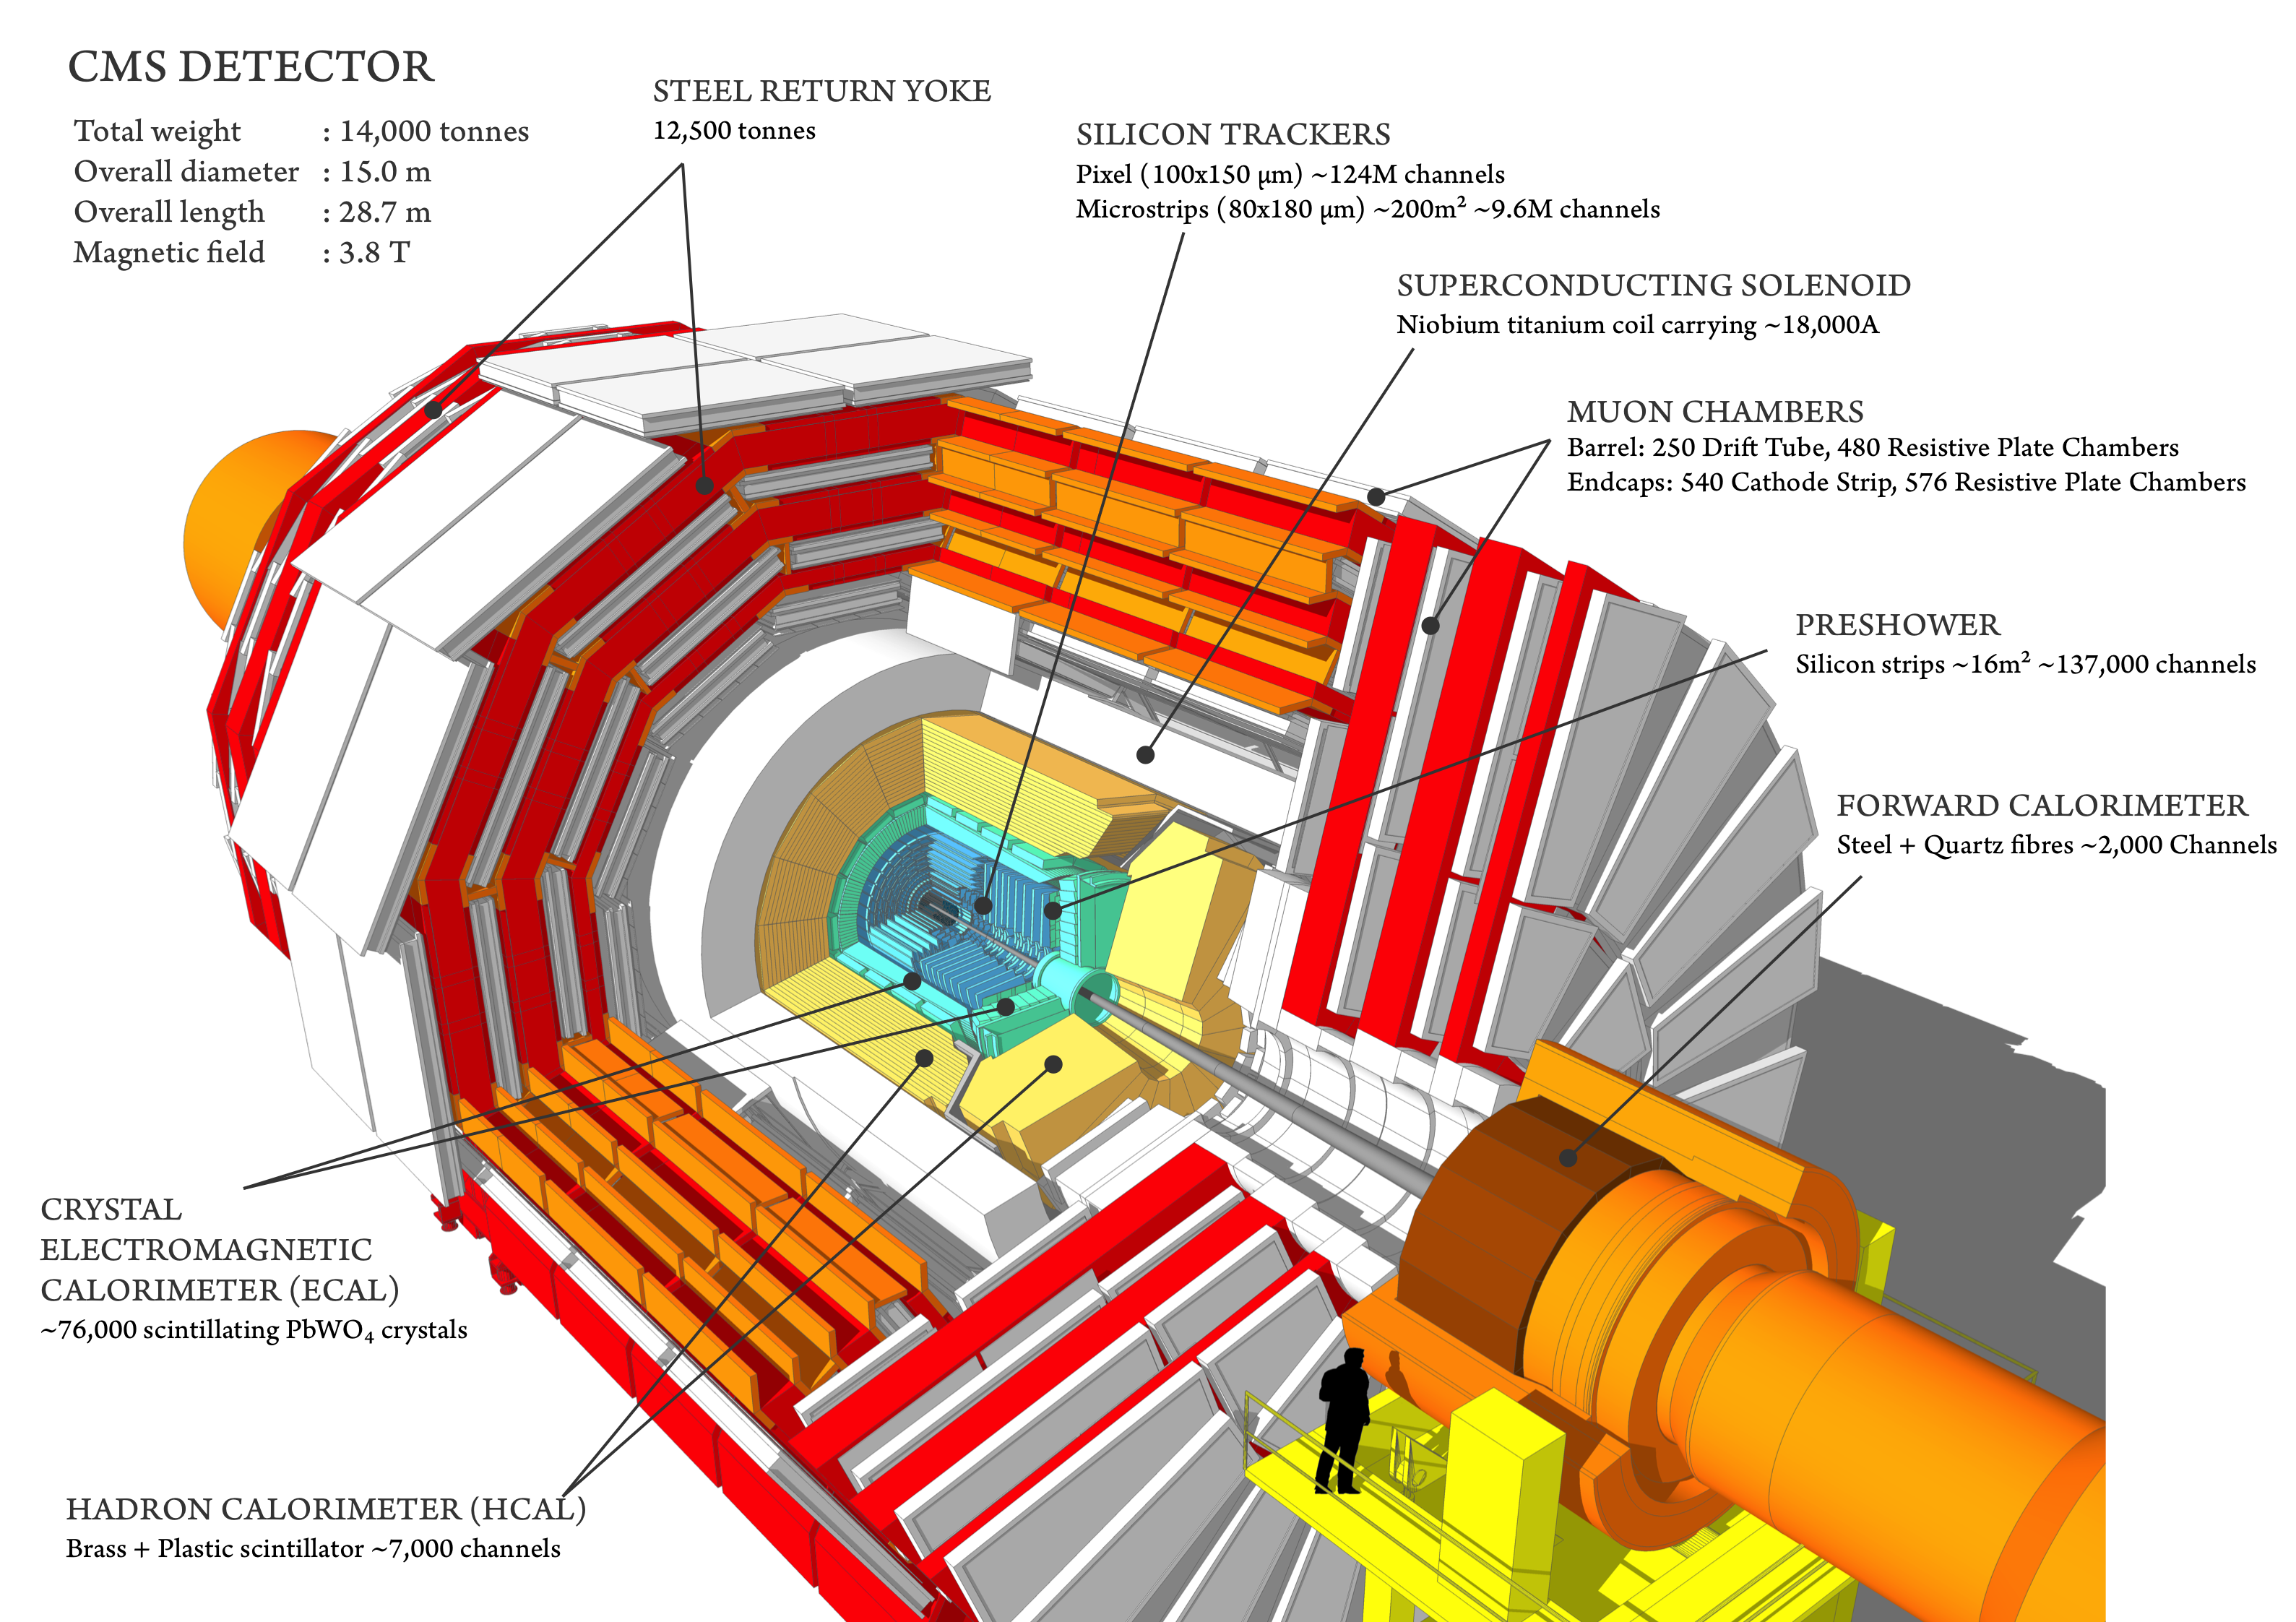
\includegraphics[width=\textwidth]{Figures/Detector/CMSschematic.png}
  \caption[A schematic view of the CMS detector.]
  {A schematic view of the CMS detector.
  Part of the detector is cut away in order to display each subsystem.
  Figure taken from Ref.~\cite{SketchUp}.}
  \label{fig:detector_CMSschematic}
\end{figure}

A cylindrical coordinate system is used to describe events within CMS, with its centre at the nominal proton-proton interaction point.
The central part is referred to as the barrel, with two endcaps closing the cylinder.
The positive $z$-axis is defined to be parallel to the beampipe in the direction of the Jura mountains, anti-clockwise when viewed from above.
The azimuthal angle $\phi$ is measured from the $z$-axis, and polar angle $\theta$ from the plane perpendicular to the $z$-axis.
Other common quantities are: pseudorapidity, defined as $\eta \, = \, -\ln{\tan{\theta/2}}$; 
momentum in the direction transverse to the plane of the LHC, \pt; 
and the magnitude of the negative vector sum of particle momenta in the transverse plane, \met.
High pseudorapidity values, corresponding to a direction close to the beampipe, are referred to as being forward.

\subsection{Solenoid}

The central feature of the CMS detector is the superconducting solenoid, whose 220 tonne cold mass is maintained at 4.5\,K.%using liquid helium cooling - 1.8K redundancy
The coil of the magnet measures 6\,m in diameter, is 13\,m long, and provides a maximum field strength of 4\,T, storing a total energy of 1.6\,GJ.
During normal operation however the current is reduced to approximately 95\% of its capacity, resulting in a field strength of 3.8\,T.
This ensures the longevity of the solenoid.
The magnetic flux is returned by a 10,000 tonne yoke, composed of three disk-like layers in both the barrel and endcaps.

The extremely high bending power of the CMS magnet enables precise measurement of charged particle tracks , 
and hence excellent momentum resolution up to very high particle momenta.
Its layout drives the design of the rest of the detector.

\subsection{Tracking}

The innermost subsystem of CMS is the silicon tracker, which is 5.8\,m long and 2.5\,m in diameter. 
Proximity to the beampipe implies the tracker must withstand a high radiation dose over its expected 10-year lifetime without degradation in performance.
It is responsible for reconstructing the curved tracks produced when charged particles are deflected by the magnetic field. %homogenous across the tracker
Furthermore, it is used to identify interaction vertices; 
this applies both for locating the primary vertex of the hard interaction and for identifying secondary vertices, produced for example in decays of $b$ quarks.
The tracker must be sufficiently granular to disambiguate tracks not only from the primary vertex but from additional pileup vertices.
Its response must also be fast enough to correctly assign tracks to the correct bunch crossing.
Finer granularity and precise timing capability require a high density of on detector electronics, and corresponding cooling capability.
This results in an increased material budget in front of the detector calorimetry, which adversely affects the achievable energy resolution; 
a compromise between the two objectives is necessary.
The final all-silicon design satisfies the requirements above, and is displayed in Figure~\ref{fig:detector_tracker}.

%TODO update this with a prettier picture
\begin{figure}[h!]
  \centering
  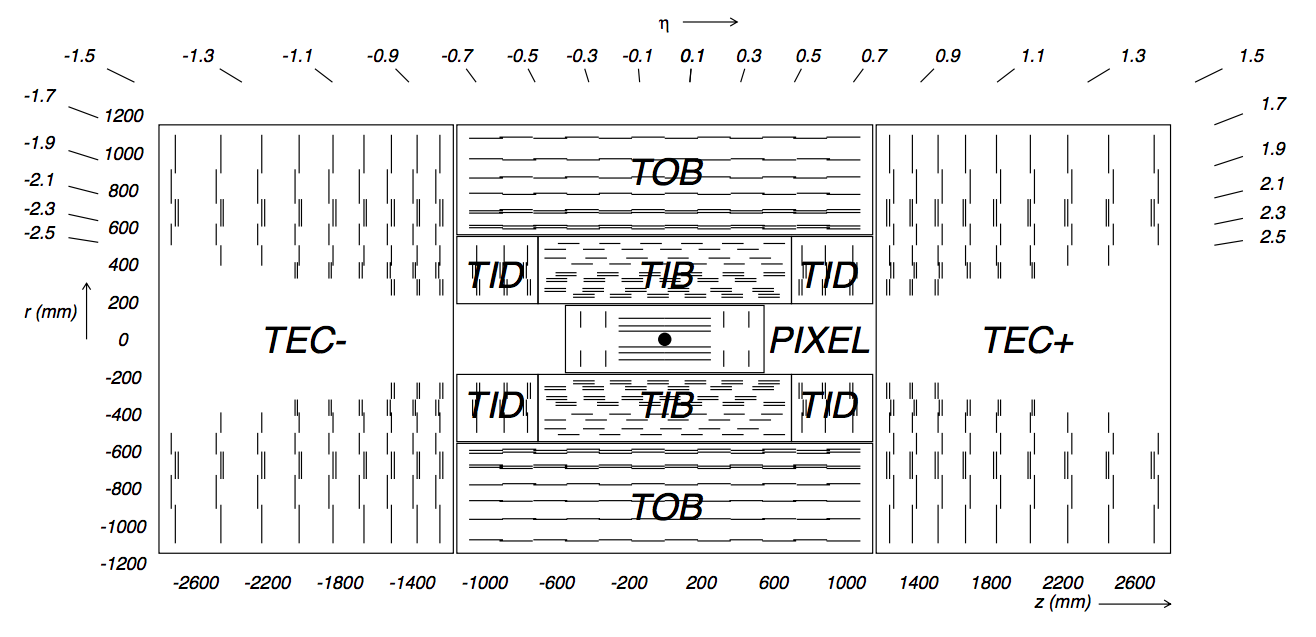
\includegraphics[width=\textwidth]{Figures/Detector/TrackerUgly.png}
  \caption[The CMS tracker.]
  {The various sections of the CMS tracking system.
  The black circle represents the nominal interaction point.
  Abbreviations are described in the following text.
  Figure taken from Ref.~\cite{CMSdetector}.}
  \label{fig:detector_tracker}
\end{figure}

The CMS tracker design comprises an inner pixel detector and a strip detector, covering the pseudorapidity range $|\eta|\,<\,2.5$.
The pixel detector provides precise two-dimensional (2D) space measurements in the $\phi$ and $z$ directions.
In the barrel, there are three modules arranged in cylindrical layers at radii of 4.4, 7.3, and 10.2\,cm. 
Two disc layers are present in each endcap, ensuring the presence of at least three tracking points across almost the full range in $\eta$.
Each cell measures $100\mu\textrm{m}\times150\,\mu\textrm{m}$, resulting in a total of 66\,million pixels covering an area of $1\,\textrm{m}^2$.
This results in an optimal position resolution of 10 and $20\,\mu\textrm{m}$ in the transverse and longitudinal direction respectively.

Beyond the pixel detector, the strip tracker provides one-dimensional measurements using 320 and $500\,\mu\textrm{m}$ thick silicon micro-strip sensors.
The strip tracker consists of three separate subcomponents, as illustrated in Figure~\ref{fig:detector_tracker}.
The Tracker Inner Barrel and Disks (TIB and TID) together consist of four barrel layers and three endcap disks, covering a radius between 20 and 55\,cm. %look up why the pitch is important
The TIB/TID provide as many as four $\phi$ measurements, depending on the track pseudorapidity.
Adjacent to the TIB/TID is the Tracker Outer Barrel (TOB), which extends up to 116\,cm in radius and 118\,cm in $z$.
A further 6 $\phi$ measurements are made in the TOB.
In both the TIB/TID and the TOB, the first two layers have a second strip module mounted back-to-back with the first, permitting a 2D measurement in $\phi-z$.
Finally the Tracker EndCaps (TECs) complete the CMS tracking apparatus.
Each has 9 disks providing a $\phi$ measurement, with the first, second and fifth containing a second module to facilitate 2D $\phi-z$ measurements.
In sum therefore, the tracker performs approximately nine measurements in the range $|\eta|\,<\,2.5$, of which around four are 2D.
It achieves a momentum resolution of better than 2\% for high \pt (100\,GeV) charged particle tracks up to $|\eta|\,=\,1.6$. %beyond this degrades due to reduced lever arm - ??
In the \Hgg analysis, the tracker plays an important role in identifying the diphoton interaction vertex. %and photon/electron ID
The low material budget also maintains the excellent intrinsic photon energy resolution of the ECAL.
%rises from 0.4 radiation lengths ($X_0$) centrally to 1,8\,$X_0$ at $|\eta|\,=1.4$, before falling to 1\,$X_0$ at $|\eta|\,=2.5$

During the year-end technical stop between 2016 and 2017, an upgraded pixel detector was installed~\cite{PixelUpgrade}.
The motivation for the upgrade was to maintain or improve existing performance despite the greater than expected instantaneous luminosities provided by the LHC.
The original pixel detector suffered from data loss at high occupancy, lower efficiency at high pileup, and degradation in performance due to radiation damage.
Key improvements in the upgraded version include a fourth layer, a new readout chip, slightly reduced material budget and greater radiation hardness.
The installation was successful and smooth operation was reached during 2017 data-taking.
Performance in several areas, such as $b$-tagging, was enhanced as a result.
However the overall impact on the \Hgg analysis was relatively small.

\subsection{Electromagnetic calorimeter}

The CMS ECAL is a homogeneous detector which uses lead tungstate (\pbw) crystals as the active material.
A total of 61200 crystals cover the barrel area (EB), with 7324 in each of the endcaps (EE).
Readout is performed by silicon avalanche photodiodes (APDs) and vacuum phototriodes (VPTs) in the barrel and endcap regions respectively.
An additional preshower detector is present in front of the endcaps, in order to improve $\pi_0$ rejection.
The total coverage in pseudorapidity reaches $|\eta|\,=\,3$; full energy resolution is maintained to ~$|\eta|\,=\,2.5$.
The ECAL is the most important sub-detector in the \Hgg analysis, 
and the ECAL design itself was driven by the need to precisely reconstruct the two photons produced in Higgs boson decays.
Hence this section is dedicated to describing the ECAL in some detail.
The overall structure is shown in Figure~\ref{fig:detector_ECALschematic}.

\begin{figure}[h!]
  \centering
  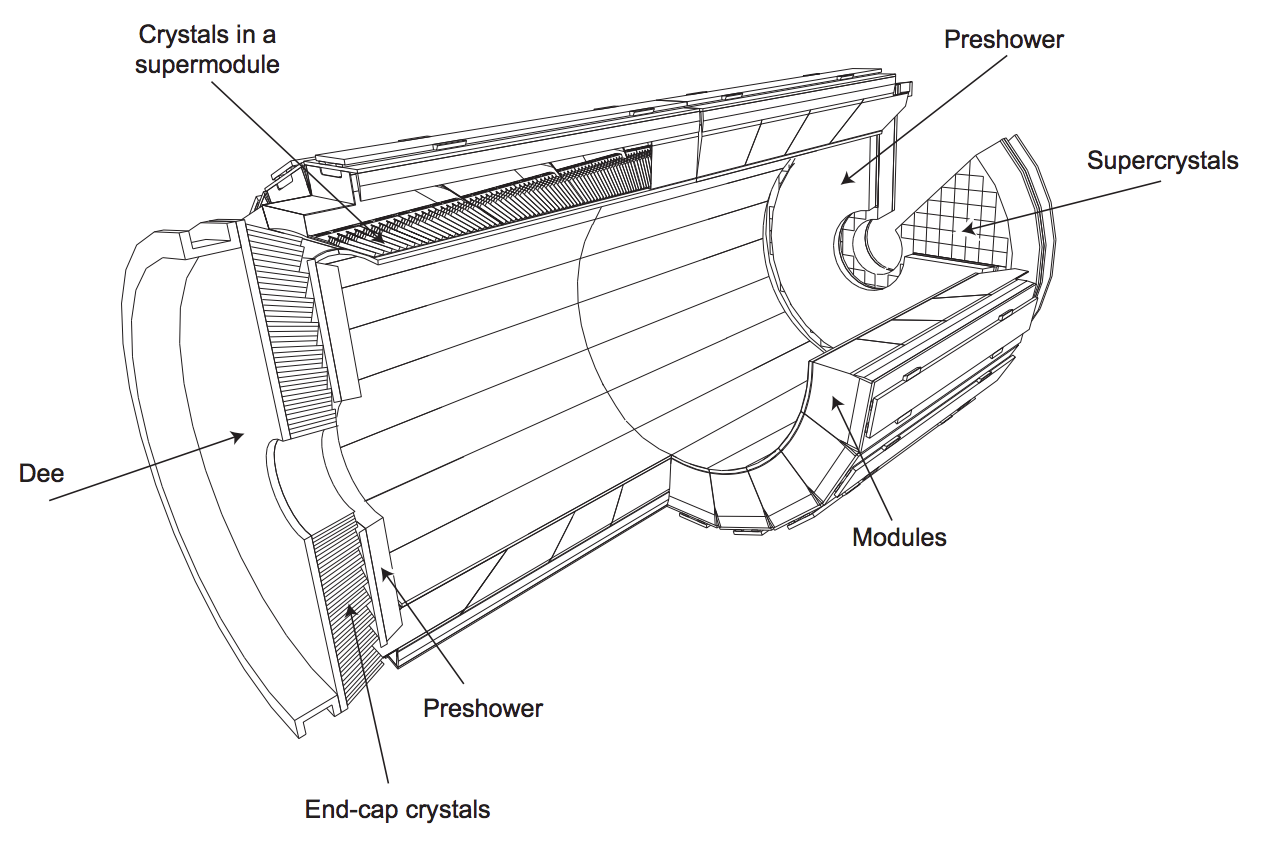
\includegraphics[width=\textwidth]{Figures/Detector/ECALschematic.png}
  \caption[Schematic view of the CMS ECAL.]
  {A schematic view of the CMS ECAL showing the various subsystems.
  Part of the detector is cut away for clarity.
  Figure taken from Ref.~\cite{ECALperformance}.}
  \label{fig:detector_ECALschematic}
\end{figure}

The choice of \pbw was motivated by the need for the active material to be fast, dense, and radiation hard.
The short response time is necessary to collect the energy deposit before the next bunch crossing; 
\pbw crystals emit approximately 80\% of the total scintillation light in 25\,ns.
Their high density (8.28\,g/$\textrm{cm}^3$) facilitates the compactness and granularity of the detector without compromising on the containment of electromagnetic showers.
A radiation length of 0.89\,cm means the 22\,cm barrel (23\,cm endcap) crystals cover a 24.7\,$X_0$ (25.8\,$X_0$) in the longitudinal direction. %mean distance travelled before reaching 1/e of original energy via brem
Lateral containment is also excellent, with a Moli\`ere radius of 2.2\,cm. %radius of cylinder containing 90% of average deposition; two contain 95% therefore.

The EB extends to $|\eta|\,=\,1.479$, as shown in Figure~\ref{fig:detector_ECALquadrant}.
Each crystal has a tapered shape which covers $0.0174\times0.0174$ in $\eta-\phi$, 
which is around $22\times22\,\textrm{mm}^2$ at the front face and $26\times26\,\textrm{mm}^2$ at the back.
The geometry is ``pseudo-projective"; the axis of each crystal is rotated by approximately $3^{\circ}$ in both $\eta$ and $\phi$ relative to the vector from the interaction point.
This ensures that a particle cannot follow a trajectory entirely within a crack in the detector.
Crystals are then grouped into supermodules, each covering $20^{\circ}$ in $\phi$.

Each EE comprises two so-called ``Dees", built from 5-by-5 supercrystals, reaching $|\eta|\,=\,3$.
The crystals in the EE are slightly shorter and wider than in the EB, 
and the offset angle varies between $2^{\circ}$ and $8^{\circ}$.
The preshower detectors (ES) in front of the endcaps are sampling calorimeters, 
each composed of two layers of lead with silicon strip sensors behind. %3X0 in total
Measurements of both energy and transverse shower shape are made by the ES.
The setup as a whole is displayed using one quadrant of the detector in Figure~\ref{fig:detector_ECALquadrant}.

\begin{figure}[h!]
  \centering
  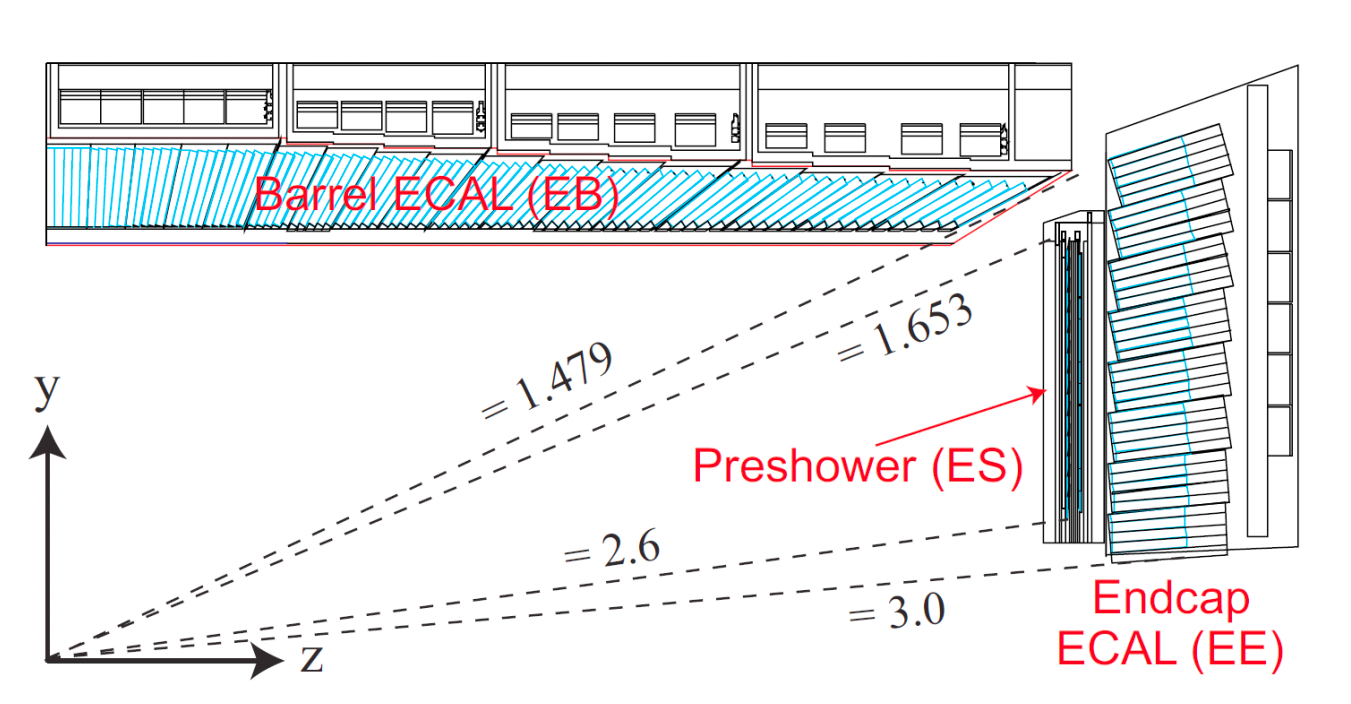
\includegraphics[width=\textwidth]{Figures/Detector/ECALquadrant.png}
  \caption[The structure in pseudorapidity of the CMS ECAL.]
  {The structure in pseudorapidity of the ECAL.
  Figure taken from Ref.~\cite{ECALperformance}.}
  \label{fig:detector_ECALquadrant}
\end{figure}

To reconstruct the shower energy, the photodetectors amplify the scintillation light to produce around 4500 photoeletrons per GeV.
After digitisation by 12-bit analogue-to-digital converters (ADCs), ten consecutive amplitude measurements are stored in a buffer.
Once a trigger is received, these recordings are sent to the off-detector electronics. 
There the original energy deposition in the crystal can be inferred with knowledge of the typical pulse shape of each channel.

The intrinsic energy resolution ($\sigma_E/E$) of the ECAL can be modelled by the equation
\begin{equation}
  \left(\frac{\sigma}{E} \right)^{2} =  
  \left(\frac{S}{\sqrt{E}} \right)^{2} +  
  \left(\frac{N}{E} \right)^{2} +  
  C^{2},
\label{eq:detector_resolution}
\end{equation}
where $S$ is the stochastic term, $N$ is the noise term and $C$ is the constant term.
%S: event-to-event fluctuations in the lateral shower containment, a photostatistics contribution of 2.1%,
%N: electronics noise, digitization noise, pileup noise.
%C: non-uniformity of the longitudinal light collection, intercalibration errors, leakage of energy from the back of the crystal.
For energy in units of GeV, the values in beam tests are found to be: %with electrons aligned with crystal centres 
$S$ = 2.8\%, $N$ = 12\%, and $C$ = 0.3\%~\cite{CMSdetector}.
Here energy values are computed simply summing $5\times5$ arrays of crystals.
In real conditions, further corrections are applied to achieve similar performance to that in beam tests.

A series of calibrations are required in order to generate accurate shower energy estimates.
Furthermore, not all the energy from a given shower will be contained within one crystal.
Typically showers are spread in the $\phi$ direction due to the effect of the magnetic field on particles produced via secondary interactions.
Therefore nearby crystals are merged into ``superclusters" (SC), 
which are then used to estimate the energy of the candidate object using the equation~\cite{ECALperformance}:
\begin{equation}
E_{e/\gamma}\, =\, F_{e/\gamma}\, G\, \Sigma_i S_i (t) C_i A_i + E_{ES}
\label{eq:}
\end{equation}
where the individual channel amplitudes ($A_i$), corrected for variations in time ($S_i (t)$) and by channel ($C_i$), 
are summed and multiplied by the global ADC-to-GeV conversion factor ($G$).
After any contribution from the preshower detector is added ($E_{ES}$), 
a final correction ($F_{e/\gamma}$) for effects due to upstream material, geometry, and imperfect clustering is applied. 
%This is the famous regression, I tihnk. So geometry = location within ECAL
The $S_i (t)$ monitor the radiation-induced change in transparency over time by measuring the response of each crystal to 440\,nm laser light every 40 minutes. %also recovers by "spontaneous annealing"
The intercalibration factors $C_i$ reflect the need to have an equal response from each crystal in the detector.
These are computed both using the $\phi-\textrm{symmetry}$ of the detector and the known mass of $\pi^{0}$ and $\eta$ diphoton decays.
The global scale $G$ is derived by requiring the measured dielectron mass of the $Z$ boson to match its known true value.
Finally, the particle-dependent $F_{e/\gamma}$ corrections are estimated using a multivariate analysis (MVA) which mostly accounts for the varying material budget in front of the ECAL.
After this lengthy procedure, the final energy resolution on the high \pt, unconverted photons which drive the \Hgg sensitivity is approximately 1\%.

\subsection{Hadronic calorimeter}

Surrounding the ECAL is the HCAL, a brass and scintillator sampling calorimeter covering the entire region $|\eta|\,<\,5$.
The HCAL measures the energy of neutral hadrons, and plays an important role in the reconstruction of jets and \met.
Four subdetectors form the full calorimeter, as illustrated in Figure~\ref{fig:detector_HCAL}.

The barrel (HB) covers the central region $|\eta|\,<\,1.3$
Wavelength-shifting fibres contained within scintillator tiles channel emitted light to photodetetors.
Division into 16 $\eta$ sectors and 16 wedges in $\phi$ results in a granularity of $0.087\times0.087$.
The HB has 14 brass layers surrounded by a layer of steel at the front and back, 
which totals between 5.8 and and 10.6 interaction lengths ($\lambda_I$) depending on $\eta$. %as a function of eta. TODO look up interaction length definition
This is not sufficient to completely contain hadronic showers, due to the space restriction imposed by the magnet coil.
Consequently an additional outer hadron calorimeter (HO) is present beyond the solenoid.
The HO uses the solenoid coil as an absorber, with the same scintillator technology as the HB.
Once the HO is taken into account, the minimum depth becomes 11.8\,$\lambda_I$, 
which significantly reduces energy leakage. % and ensures a Gaussian energy profile for neutral hadrons.

The hadronic endcaps (HE) reach across a wide pseudorapidity range, covering $1.3\,<\,|\eta|\,<\,3.0$.
This more forward region requires highly radiation hard material, for which reason brass is chosen. %also because not magnetic
The HE design minimises the size of the barrel-endcap transition region, and results in a depth of at least 10\,$\lambda_I$.
Its granularity matches the HB up to $\eta\,=\,1.6$, but reduces to $0.17\times0.17$ beyond that.

Finally, the very forward region contains the HF (forward calorimeter).
Its design is driven primarily by the need to withstand an extremely high radiation dose.
Good performance must also be maintained, since the HF plays an important role in forward jet reconstruction, which occurs for example in VBF \Hgg events.
The chosen active material is quartz fibre, with a steel absorber structure.
The fibres generate light via Cherenkov radiation, which is detected by photomultipliers.
Fibres are bundled together with a granularity of $0.175\times0.175$.
Two different lengths of fibre are utilised; 
around half run the full length of the HF, whilst the other half begin at a depth of 22cm from the HF front face.
%Almost all the the energy of an electron or photon is deposited in the first half, 
%whereas a hadronic object will produce approximately equal signals in each half.
This enables electromagnetic showers to be disambiguated from hadronic showers.
%TODO Parameters of the CMS HCAL, following Equation~\ref{eq:resolution}, are...

\begin{figure}[h!]
  \centering
  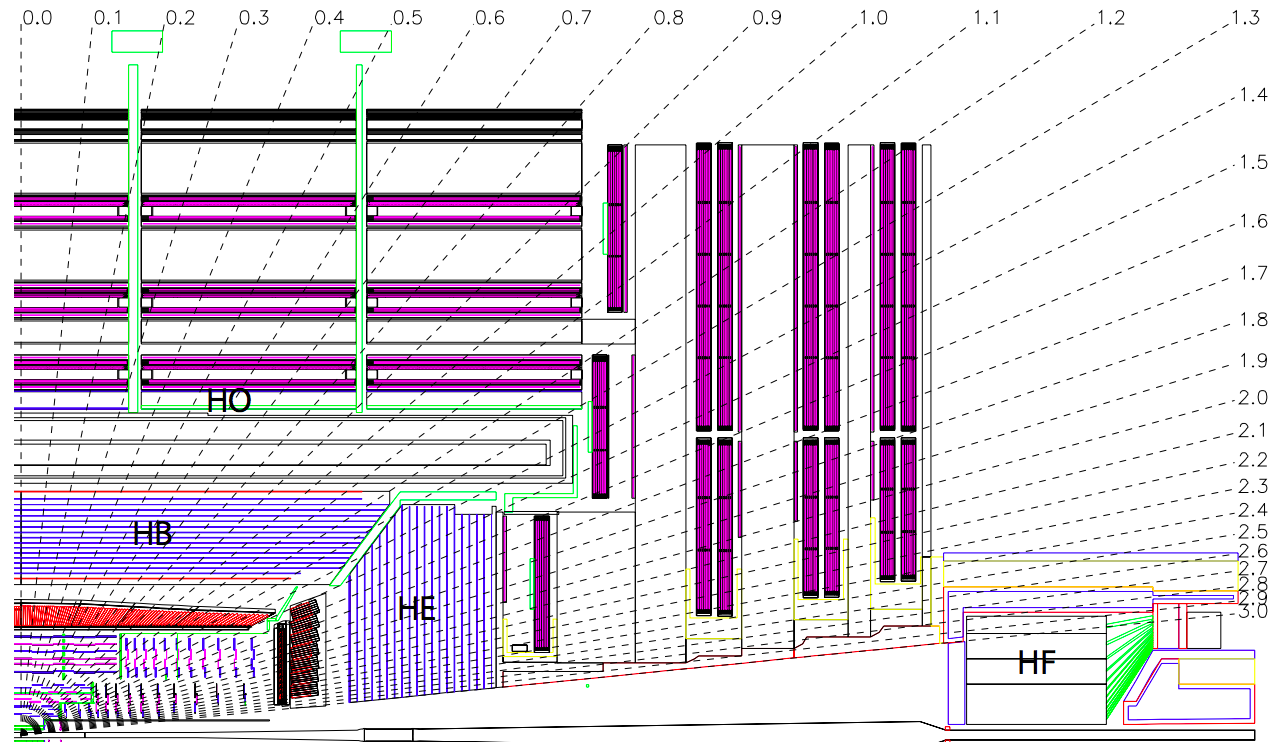
\includegraphics[width=\textwidth]{Figures/Detector/HCAL.png}
  \caption[The structure in pseudorapidity of the CMS HCAL.]
  {The structure in pseudorapidity of the HCAL.
  Figure taken from Ref.~\cite{CMSdetector}.}
  \label{fig:detector_HCAL}
\end{figure}

\subsection{Muon system}

The muon system at CMS is composed of three separate gaseous chamber detectors.
The system is required to identify muons, precisely measure their momentum, and inform the triggering decision.
Good muon performance is crucial to the success of CMS, particularly for the very powerful $H \rightarrow ZZ^* \rightarrow 4\mu$ decay mode.
Interleaved with the return yoke of the CMS magnet, the muon system comprises a cylindrical barrel system and two endcap planes, 
covering a total area of 25000\,$\textrm{m}^2$.

The barrel drift tube (DT) covers the central region up to $|\eta|\,=\,1.2$ with four layers, known as stations, between layers of the return yoke.
Drift chambers containing a mixture of Ar and $\textrm{CO}_2$ gases are used; this is possible due to the low rate and uniform magnetic field in the barrel region.
Each station has eight chambers providing a measurement of the $\phi$ direction and four measuring the $z$ coordinate.
At high \pt, the identification efficiency using the DT alone is over 95\%.

In the endcap region there is both a higher muon rate and higher neutron background, which necessitates the use of a more radiation hard technology. %and the magnetic field less uniform
The four Cathode Strip Chamber (CSC) stations overlap with the DT from $0.9\,<|\eta|\,=\,1.2$.
Beyond this, a muon will pass through at least three CSCs between $\eta\,=\,1.2$ and $\eta\,=\,2.4$.
The CSCs have fast timing capability, which enables them to inform the trigger and also correctly identify the bunch crossing with efficiency greater than 99\%.

The final component of the muon system is the Resistive Plate Chamber (RPC) system.
The six RPC layers are embedded within the DT but operate independently.
Position resolution is coarser, but the timing resolution is fast.
This facilitates a complementary trigger input, as well as helping to remove track ambiguities arising from multiple hits in a single chamber. % especially good for low pT tracks which don't reach further back stations

Overall, the muon system alone achieves a momentum resolution of around 10\% for central muons up to $\pt=200\,\textrm{GeV}$.
This worsens to between 15\% and 40\% for 1\,TeV muons, dependent on pseudorapidity.
Once combined with the information from the tracker however, this improves to 5\% in the barrel and 10\% in the endcaps.

Summarising the lateral structure of CMS, 
Figure~\ref{fig:detector_CMSslice} shows the characteristic paths followed by the different types of particles produced in LHC proton-proton collisions.

\begin{figure}[h!]
  \centering
  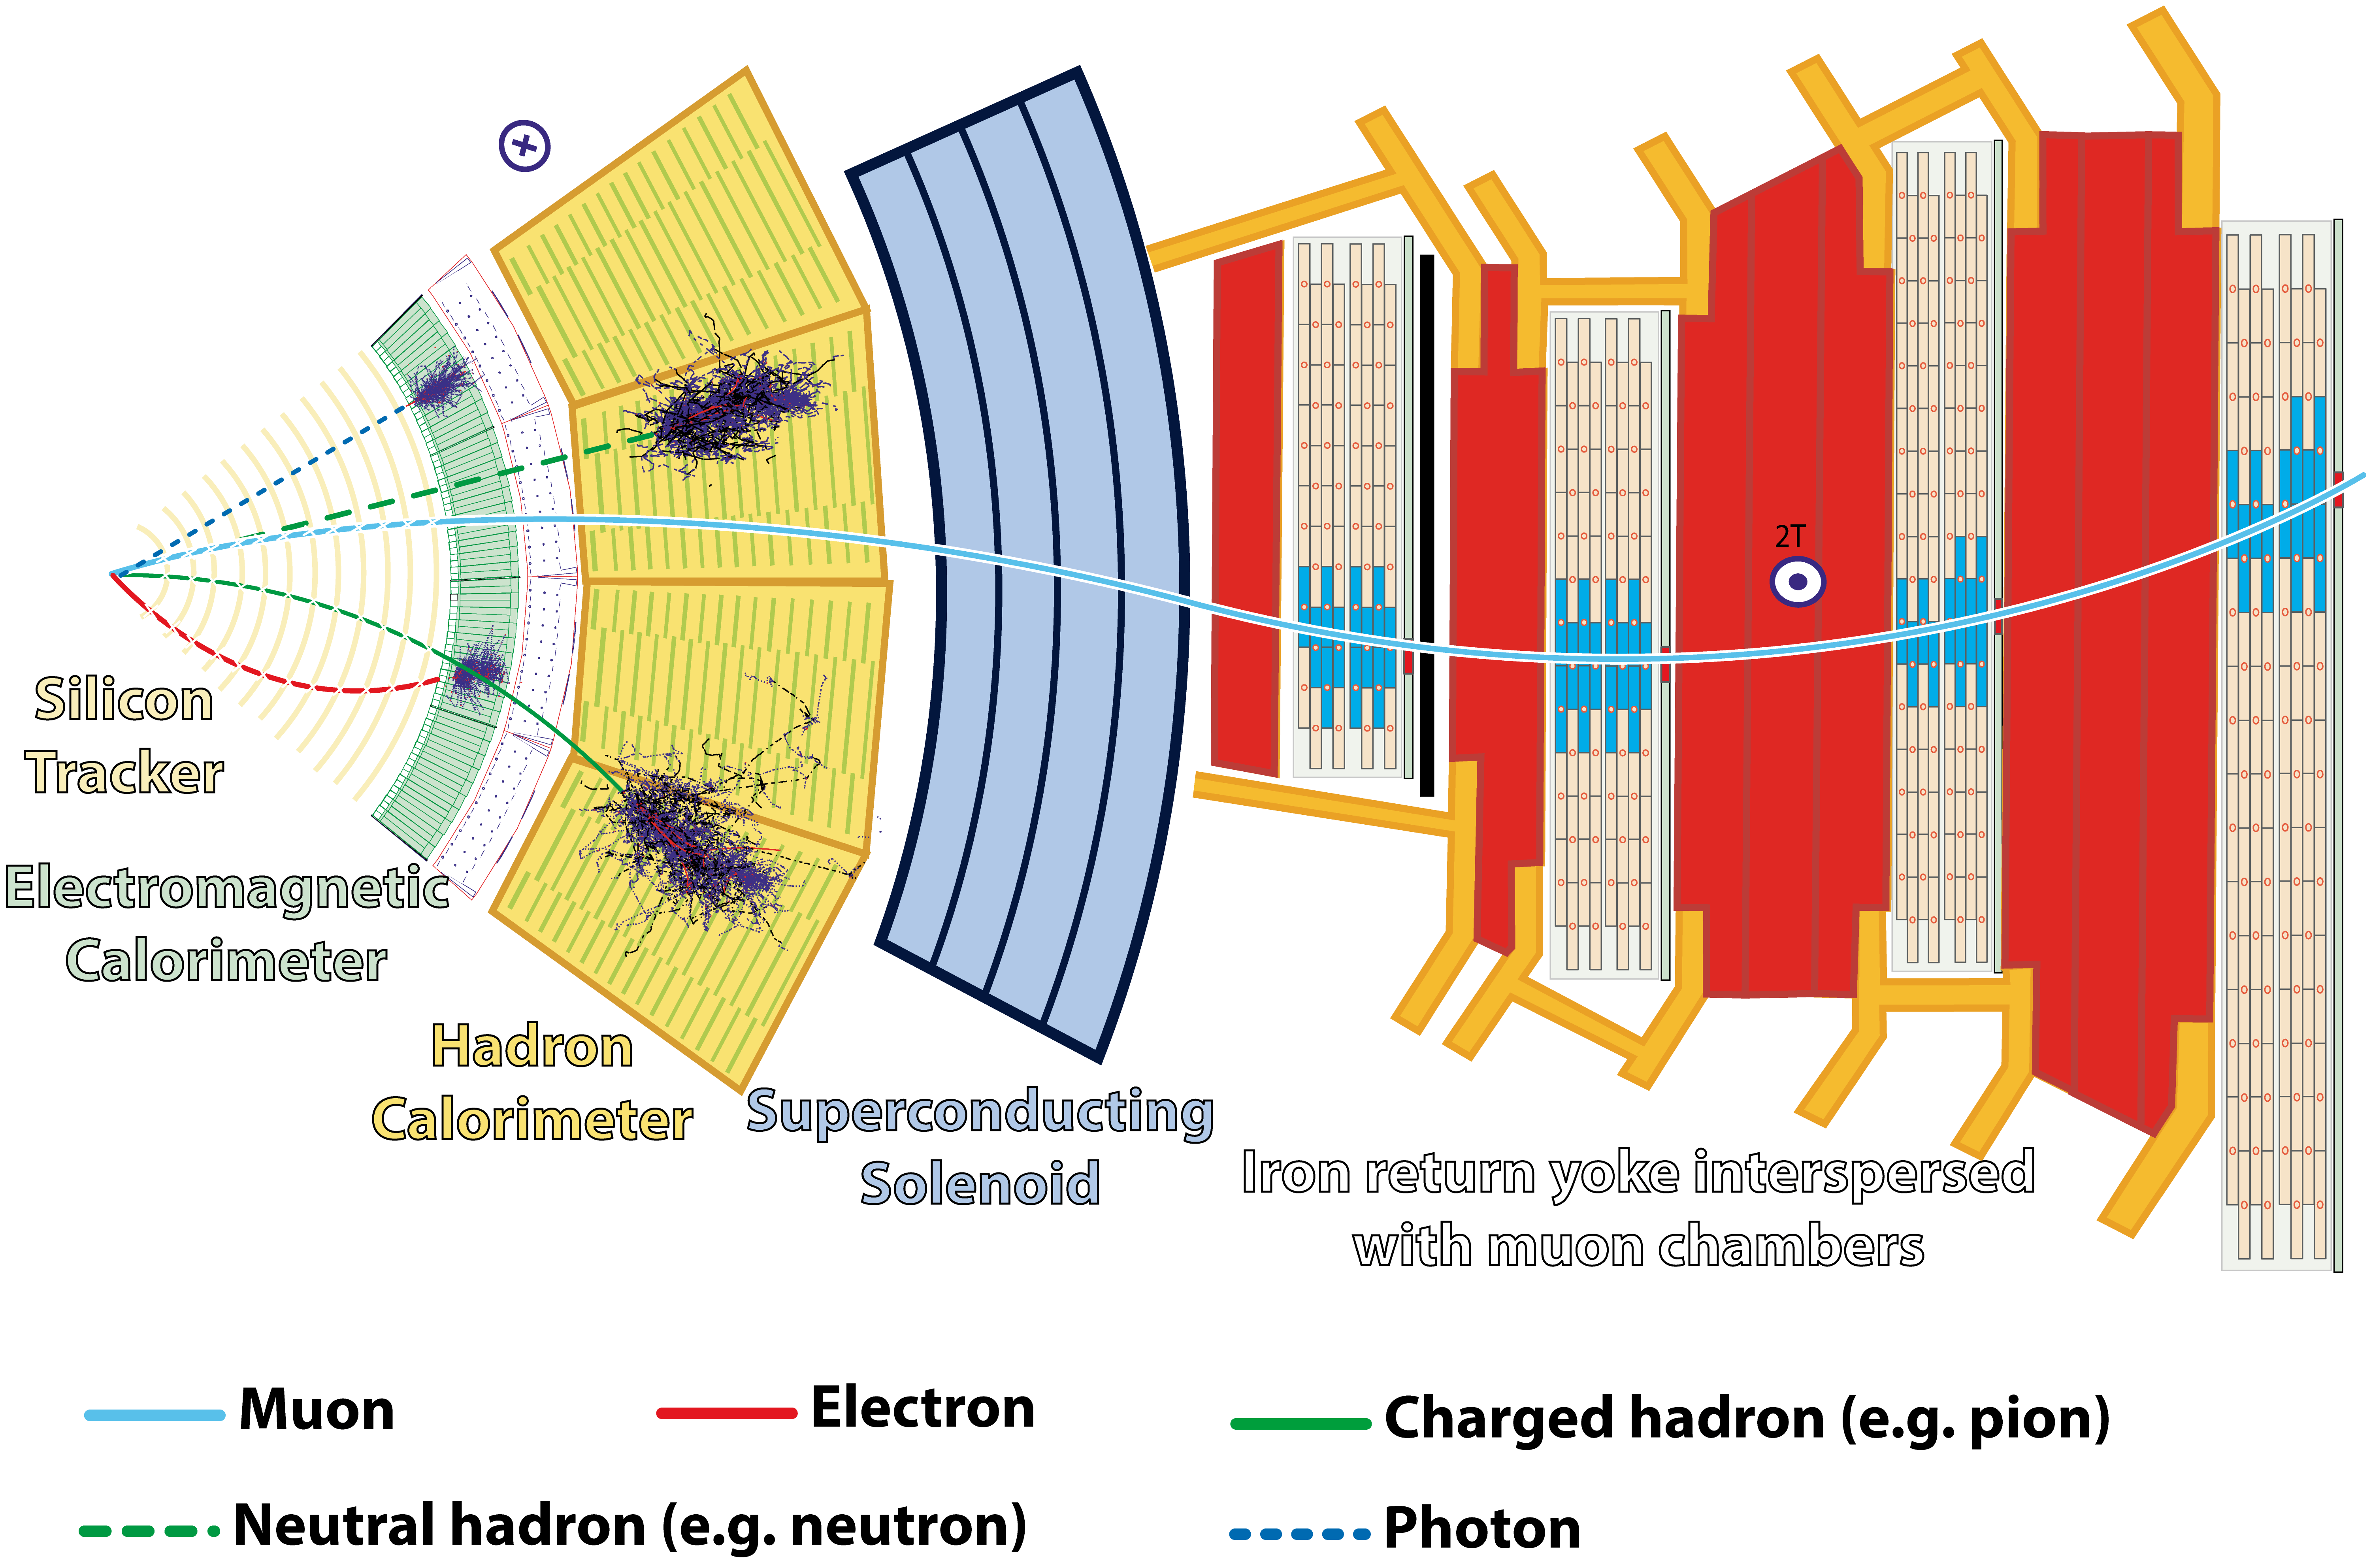
\includegraphics[width=\textwidth]{Figures/Detector/CMSslice.png}
  \caption[A cross-sectional view of the CMS detector]
  {A cross-sectional view of a slice of the CMS detector, 
  illustrating the path of a muon (blue line) 
  and the muon chambers interleaved with the return yoke.
  Figure taken from Ref.~\cite{CMSslice}.}
  \label{fig:detector_CMSslice}
\end{figure}

\subsection{Trigger system}

The rate of information produced at CMS is extremely high; the bunch crossings occurring at rate of 40\,MHz each contain ~1\,MB of data.
It is unfeasible to read out 40\,TB of data per second, so a drastic reduction in the event rate must be applied.
This is achieved by ignoring the large majority of events where the protons collide at a relatively low angle and no high energy objects are produced as a result.
The system responsible for this rate reduction is known as the trigger.

The CMS trigger runs in two sequential stages: first the Level-1 Trigger (L1T) and then the High-Level Trigger (HLT).
Since the maximum output rate of the detector electronics is 100\,kHz, the L1T is responsible for a factor 400 decrease in the number of events selected.
The L1T must make a decision on an event within approximately $3.2\,\mu s$, and therefore only uses a coarse readout of data from the calorimeters and muon system.
The full resolution interpretation of an event is buffered until the final trigger decision is made. %total of 128 bunch crossings stored in buffer!!
Simple algorithms, for example the energy sum from arrays within a calorimeter, are used to identify high energy objects of interest.
The computations necessary are performed mostly by customised, reprogrammable electronics known as Field Programmable Gate Arrays (FPGAs).
Once a decision has been made, if the event passes the L1T selection, the full readout is transmitted to the HLT.

The HLT is a software system which runs on a single farm of commercially available processors. %about 16,000 CPU cores
It must further reduce the event rate to 1\,kHz, which corresponds to a factor of ~100.
As the HLT has access to the full event information, sophisticated reconstruction algorithms similar to those used offline are employed. 
It must maintain selection efficiency whilst maintaining an acceptable rate and CPU-time. 
Typical quantities evaluated to inform HLT decisions include invariant mass, object isolation, and track information.
Finally, once the HLT has accepted an event, the full readout is saved to disk.
The event is then processed by the full offline CMS software, which produces objects ready for physics analysis.
